\chapter{Численное моделирование гидродинамических задач смазочного слоя}

\section{Граничные условия}
Для замыкания дискретной задачи необходимо задать граничные условия на давление~$p$ и (при использовании модели JFO) на степень заполнения~$\vartheta$. Тип граничных условий определяется физической постановкой (подразделы~2.1.2-2.1.4) и геометрией расчётной области. Ниже систематизированы три основных типа граничных условий для давления.

\textit{Дирихле (заданное давление).}
На соответствующем участке границы $\Gamma_D$ давление фиксируется:
\[
  p = p_0 \quad \text{на} \quad \Gamma_D.
\]

Наиболее распространённый случай -- $p_0 = p_{\mathrm{cav}} = 0$ (в избыточных давлениях) на открытых границах расчётной области, где смазочный слой сообщается с окружающей средой. Типичные примеры: торцы по оси~$z$ для радиального подшипника, радиальные границы $r = R_{\mathrm{in}},\, R_{\mathrm{out}}$ для упорного.

\textit{Периодичность.}
По окружному (периодическому) направлению давление совпадает на противоположных границах области:
\[
  p(x_{1,s},\, x_2) = p(x_{1,t},\, x_2).
\]

Данное условие применяется в упорных и радиальных подшипниках, где расчётная область охватывает полный период по окружной координате. При расчёте сектора вместо периодичности на границах сектора задаются условия симметрии ($\partial p / \partial n = 0$) или заданное давление в зависимости от постановки.

\textit{Непроницаемость (Нейман).}
На участках с условием симметрии или непроницаемости нормальная производная давления обращается в нуль:
\[
  \frac{\partial p}{\partial n} = 0 \quad \text{на} \quad \Gamma_N.
\]

Условие $\partial p / \partial n = 0$ эквивалентно отсутствию напорного потока через границу и используется на линиях симметрии или на искусственных границах при расчёте сектора.

В таблице~\ref{tab:bc_summary} сведены граничные условия для давления, соответствующие трём постановкам, сформулированным в подразделах~2.1.2-2.1.4.

\begin{table}[!ht]
\centering
\caption{Граничные условия для давления в различных постановках
  (координаты $x_1$,~$x_2$ определены в подразделах~2.1.6 и~2.2.1)}
\label{tab:bc_summary}
\begin{tabularx}{\textwidth}{|X|c|c|}
\hline
\multicolumn{1}{|c|}{\textbf{Постановка}} & \textbf{По $\boldsymbol{x_1}$}
                       & \textbf{По $\boldsymbol{x_2}$} \\
\hline
Торцевой зазор
  & периодичность
  & $p = p_{\mathrm{cav}}$, $x_2 = r$ \\
\hline
Радиальный зазор при окружном сдвиге
  & периодичность
  & $p = p_{\mathrm{cav}}$, $x_2 = z$ \\
\hline
Радиальный зазор при возвратно-поступательном движении
  & $p = p_{\mathrm{cav}}$, $x_1 = z$
  & периодичность \\
\hline
\end{tabularx}
\end{table}

\FloatBarrier

При использовании массо-сохраняющей модели кавитации JFO (раздел~2.3) дополнительно задаются граничные условия на степень заполнения~$\vartheta$. На границах подачи смазки полагается $\vartheta = 1$ (полное заполнение зазора). По периодическим направлениям степень заполнения периодична, аналогично давлению. На выходных границах с $p = p_{\mathrm{cav}}$ величина~$\vartheta$ явно не фиксируется; она определяется из уравнения сохранения~\eqref{eq:jfo_conservation} и схемы переноса, что соответствует свободному выходу смеси.

Во всех рассматриваемых постановках кавитационное давление принимается равным нулю в избыточных давлениях: $p_{\mathrm{cav}} = 0$.

Перечисленные типы граничных условий по-разному реализуются
в сеточной схеме. Узлы с условием Дирихле исключаются
из итерационного обновления: их значения фиксируются
и при вычислении потоков на соседних гранях используются
как известные. Периодичность по координатe~$s_1$ реализуется
отождествлением узлов на противоположных границах расчётной
области~-- фактически граница «замыкается» в кольцо,
и узел $i = 0$ совпадает с узлом $i = N_1$. Условие
неотрицательности давления ($P \geq 0$, кавитация
Рейнольдса) обеспечивается операцией усечения после каждого
шага SOR: если обновлённое значение оказывается отрицательным,
оно принудительно полагается равным нулю. Это эквивалентно
упрощённому методу активного множества без пересчёта степени
заполнения~$\vartheta$. Для JFO-постановки трактовка
кавитационной границы принципиально иная: граница является
свободной и определяется из условия непрерывности потока;
её поточечное обновление описано в разделе~3.5.

\textit{Физический смысл периодичности и~её~отличие от~искусственных граничных условий.}
Условие периодичности по~окружной координате является не~искусственным техническим приёмом, а~точным отражением физической геометрии задачи. Для~радиального подшипника окружная координата~$\varphi$ пробегает полный период $[0, 2\pi]$, и~давление на~входе в~расчётную область действительно равно давлению на~выходе~-- обе~<<границы>> на~самом деле описывают одно и~то~же физическое сечение. Это отличает условие периодичности от~условий Дирихле или~Неймана, которые описывают реальные физические границы (открытые торцы, стенки). Нарушение условия периодичности (например, замена его~на~условие постоянного давления на~обеих граничных линиях~$\varphi = 0$ и~$\varphi = 2\pi$) привело бы к~существенно неверным результатам, так как~фактически изменило бы топологию задачи.

\textit{Граница кавитации в~JFO-постановке как~свободная граница.}
В~упрощённых моделях кавитации (обнуление давления, модель Гюмбеля) граница кавитации явно не~выделяется: давление просто обнуляется поточечно в~тех~узлах, где оно~оказывается отрицательным. Никакого специального граничного условия на~линии раздела зон не~задаётся~-- эта линия неявно определяется самим алгоритмом обнуления.

В~JFO-постановке граница кавитации является свободной границей в~математическом смысле: её~положение не~фиксируется заранее, а~определяется в~ходе решения как~часть ответа. На~этой границе должны выполняться одновременно два условия: давление равно кавитационному~($p = p_{\mathrm{cav}}$) и~поток массы через границу непрерывен (баланс~\eqref{eq:jfo_couette_balance} из~раздела~3.5). Именно второе условие является дополнительным по~сравнению с~упрощёнными моделями и~обеспечивает выполнение баланса масс. Численно свободная граница отслеживается неявно через обновление активного множества~-- алгоритм, описанный в~разделах~2.3.3 и~3.5,~-- без явного хранения координат линии раздела зон~\cite{hori2002,szeri1998}.


\FloatBarrier
\section{Дискретизация}
Дискретизации подлежат уравнение Рейнольдса (при полном заполнении зазора) и его обобщение JFO~\eqref{eq:jfo_conservation}. В обоих случаях используется консервативная (потоковая) форма записи: для каждой ячейки формулируется баланс потоков через её грани. Такой подход обеспечивает сохранение массы на дискретном уровне и является удобной основой для реализации JFO-условий в кавитационной зоне.

Расчётная область покрывается прямоугольной равномерной сеткой с узлами~$(i,\,j)$ и шагами~$\Delta x_1$,~$\Delta x_2$ (формула~\eqref{eq:jfo_grid} в главе~2). Потоки вычисляются на гранях ячеек: $i \pm 1/2$ по~$x_1$ и $j \pm 1/2$ по~$x_2$. Граничные условия на сетке реализуются в соответствии с разделом~3.1.

Консервативный баланс массы на ячейке~$(i,\,j)$ записывается в виде
\begin{equation}\label{eq:discrete_balance}
  \frac{(\vartheta h)_{i,j}^{n+1} - (\vartheta h)_{i,j}^{n}}{\Delta t}
  + \frac{F_{i+\frac{1}{2},j} - F_{i-\frac{1}{2},j}}{\Delta x_1}
  + \frac{G_{i,j+\frac{1}{2}} - G_{i,j-\frac{1}{2}}}{\Delta x_2}
  = 0,
\end{equation}
\begin{conditions}
$F = F_P + F_C$ -- суммарный поток через грань по~$x_1$ (напорный и переносной);\\
$G = G_P + G_C$ -- аналогичный поток по~$x_2$.
\end{conditions}
При полном заполнении ($\vartheta = 1$) уравнение~\eqref{eq:discrete_balance} сводится к классической дискретизации уравнения Рейнольдса. В стационарной постановке член по времени опускается.

\textit{Напорный (пуазейлевский) поток.}
Коэффициент проводимости определяется как
\[
  K = \frac{h^3}{12\mu}.
\]

Потоки на гранях аппроксимируются центральными разностями:
\begin{equation}\label{eq:flux_poiseuille}
\begin{split}
  &F_{P,\,i+\frac{1}{2},j} = -K_{i+\frac{1}{2},j}\,
    \frac{p_{i+1,j} - p_{i,j}}{\Delta x_1}, \\
  &G_{P,\,i,j+\frac{1}{2}} = -K_{i,j+\frac{1}{2}}\,
    \frac{p_{i,j+1} - p_{i,j}}{\Delta x_2}.
\end{split}
\end{equation}

Коэффициент~$K$ на грани вычисляется усреднением значений в соседних узлах (арифметическое или гармоническое усреднение); при достаточно мелкой сетке различия между арифметическим и гармоническим усреднением, как правило, малы.

\textit{Переносной (куэттовский) поток.}
Для уравнения JFO переносной поток записывается в виде
\begin{equation}\label{eq:flux_couette}
\begin{split}
  &F_{C,\,i+\frac{1}{2},j} = \frac{\vartheta_{\mathrm{up}}\,
    h_{i+\frac{1}{2},j}}{2}\,U_1, \\
  &G_{C,\,i,j+\frac{1}{2}} = \frac{\vartheta_{\mathrm{up}}\,
    h_{i,j+\frac{1}{2}}}{2}\,U_2,
\end{split}
\end{equation}

Значение $\vartheta_{\mathrm{up}}$ выбирается из наветренного узла: при $U_1 \geq 0$ берут $\vartheta_{\mathrm{up}} = \vartheta_{i,j}$, иначе $\vartheta_{\mathrm{up}} = \vartheta_{i+1,j}$; аналогично по~$x_2$: при $U_2 \geq 0$ берут $\vartheta_{\mathrm{up}} = \vartheta_{i,j}$, иначе $\vartheta_{\mathrm{up}} = \vartheta_{i,j+1}$. При полном заполнении ($\vartheta = 1$) множитель~$\vartheta_{\mathrm{up}}$ обращается в единицу. Толщина~$h$ на грани вычисляется арифметическим усреднением. Схема расчётной ячейки с указанием потоков на гранях показана на рисунке~\ref{fig:cell_fluxes}.

\begin{figure}[!ht]
\centering
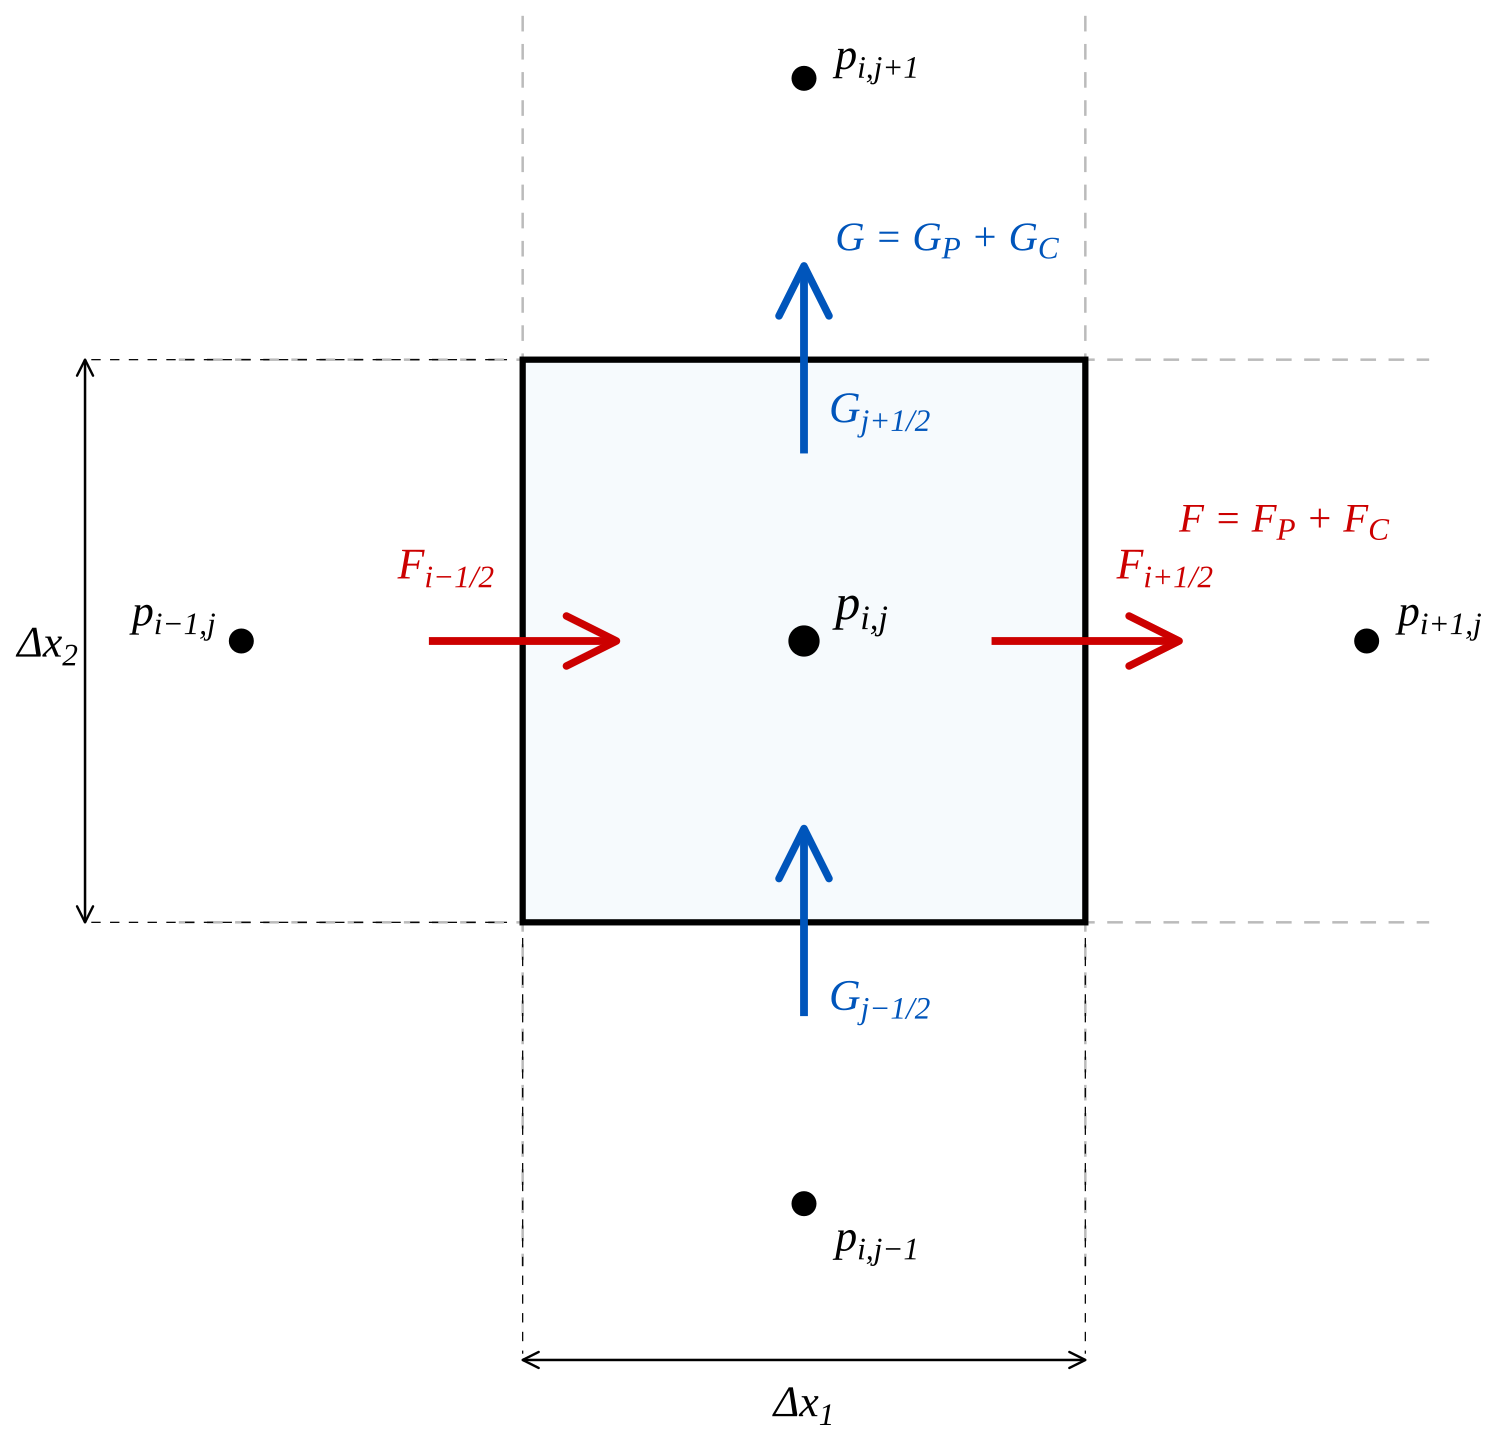
\includegraphics[width=\textwidth,height=0.9\textheight,keepaspectratio]{figures/ch03/fig_3_1.png}
\caption{Схема расчётной ячейки и потоков на гранях}
\label{fig:cell_fluxes}
\end{figure}

\FloatBarrier

\textit{5-точечный шаблон для давления.}
Подстановка потоков в баланс~\eqref{eq:discrete_balance} при $\vartheta = 1$ (стационарный случай) приводит к линейной системе вида
\begin{equation}\label{eq:5point_stencil}
  a_P\,p_{i,j} = a_E\,p_{i+1,j} + a_W\,p_{i-1,j}
    + a_N\,p_{i,j+1} + a_S\,p_{i,j-1} + b_{i,j},
\end{equation}
\begin{conditions}
$a_E$,~$a_W$,~$a_N$,~$a_S$ -- коэффициенты, определяемые проводимостями~$K$ на соответствующих гранях;\\
$a_P = a_E + a_W + a_N + a_S$ -- диагональный коэффициент;\\
$b_{i,j}$ -- правая часть, содержащая вклад куэттовского потока (и, при нестационарности, члена по времени).
\end{conditions}
Система~\eqref{eq:5point_stencil} решается итерационно; выбор решателя описан в разделе~3.3. В нестационарной постановке временной член в~\eqref{eq:discrete_balance} приводит к модификации диагонального коэффициента и правой части разностного уравнения.

В модели JFO давление в кавитационных узлах фиксируется на уровне $p_{\mathrm{cav}}$, поэтому $\nabla p = 0$ и напорные потоки в кавитационной зоне отсутствуют. Обновление активного множества и вычисление~$\vartheta$ в кавитации описаны в разделе~3.5.

Центральные разности для напорного потока обеспечивают второй порядок аппроксимации. Upwind-схема для переноса~$\vartheta$ имеет первый порядок, однако гарантирует устойчивость при доминировании конвективного переноса.

\textit{Порядок аппроксимации и влияние сетки.}
Центральные разности для напорного
потока~\eqref{eq:flux_poiseuille} обеспечивают второй порядок
аппроксимации по $\Delta x_1$, $\Delta x_2$ в узлах, где
зазор $h$ гладко изменяется. В области детерминированных
микроструктур поверхности зазор имеет резкие перепады
на границах элементов рельефа: на переднем склоне лунки $h$
возрастает, на заднем убывает на масштабе нескольких ячеек
сетки. В таких зонах локальный порядок аппроксимации снижается
до первого. Практическое следствие: для корректного
воспроизведения гидродинамического эффекта отдельного элемента
микрорельефа требуется не менее 8--10 узлов на один элемент
вдоль каждого направления. При недостаточном разрешении
коэффициент проводимости~$K_{i+1/2,\,j} =
h_{i+1/2,\,j}^3/(12\mu)$ на грани между «лункой»
и «площадкой» усредняется избыточно, что занижает контраст
потоков и уменьшает расчётный гидродинамический эффект.

\textit{Особенности схемы для цилиндрических координат.}
Для упорного подшипника расчётная область задаётся
в цилиндрических координатах $(r,\,\theta)$. Уравнение
Рейнольдса в этих координатах содержит дополнительные
множители $r$ (перед радиальным потоком) и $1/r$ (перед
угловым): характерные коэффициенты проводимости принимают вид
$K_{r} = r\,h^3/(12\mu)$ и $K_\theta = h^3/(12\mu\,r)$.
В консервативной форме~\eqref{eq:discrete_balance} это
приводит к тому, что коэффициенты~$a_E$, $a_W$ по радиальному
направлению пропорциональны $r_{i+1/2}$ и $r_{i-1/2}$
соответственно, тогда как $a_N$, $a_S$ по угловому делятся
на $r_i$. Структура пятиточечного
шаблона~\eqref{eq:5point_stencil} сохраняется, изменяются
только численные значения коэффициентов.
Правая часть~$b_{i,j}$ включает куэттовский вклад от поворота
диска и согласована с нестационарным членом при наличии
squeeze-эффекта~\cite{han2016,panday2012}.


\FloatBarrier
\section{Итерационные решатели}
Дискретизация уравнения Рейнольдса (раздел~3.2) при полном заполнении зазора ($\vartheta = 1$, стационарный случай) приводит к линейной системе~\eqref{eq:5point_stencil} с пятиточечным шаблоном. Матрица этой системы разреженная; для внутренних узлов каждая строка содержит не более пяти ненулевых коэффициентов (5-точечный шаблон). Число неизвестных определяется числом внутренних узлов сетки~$N_1 \times N_2$. Коэффициенты $a_E$,~$a_W$,~$a_N$,~$a_S$ неотрицательны, поскольку проводимость $K = h^3/(12\mu) > 0$, а диагональное преобладание $a_P = a_E + a_W + a_N + a_S$ обеспечивает благоприятные свойства системы и способствует сходимости стационарных итерационных методов. Прямые методы (например, LU-разложение) для больших сеток неэффективны из-за заполнения разреженной структуры, поэтому используются итерационные методы, допускающие поточечное обновление.

\textit{Метод Гаусса–Зейделя.}
Метод Якоби (одновременное обновление всех узлов по значениям предыдущей итерации) для уравнения Рейнольдса практически не применяется из-за медленной сходимости; его естественное улучшение~-- метод Гаусса–Зейделя. Формула обновления имеет вид
\begin{equation}\label{eq:gs_update}
  p_{i,j}^{(m+1)} = \frac{1}{a_P}\bigl(
    a_E\,p_{i+1,j}^{(m)} + a_W\,p_{i-1,j}^{(m+1)}
    + a_N\,p_{i,j+1}^{(m)} + a_S\,p_{i,j-1}^{(m+1)}
    + b_{i,j}\bigr),
\end{equation}
\noindent где верхний индекс~$(m)$~-- номер итерации. При последовательном обходе сетки по строкам значения $p_{i-1,j}$ и $p_{i,j-1}$ уже обновлены на текущей итерации (индекс~$m+1$), что ускоряет сходимость по сравнению с методом Якоби. Узлы с условиями Дирихле не обновляются~-- их значения фиксированы (раздел~3.1). Периодичность учитывается связыванием пар узлов на противоположных границах расчётной области.

\textit{Последовательная верхняя релаксация (SOR).}
Для ускорения сходимости вводится параметр релаксации~$\omega$. Обновление выполняется в два шага:
\begin{equation}\label{eq:sor_update}
\begin{split}
  &\tilde{p}_{i,j} = \frac{1}{a_P}\bigl(
    a_E\,p_{i+1,j}^{(m)} + a_W\,p_{i-1,j}^{(m+1)}
    + a_N\,p_{i,j+1}^{(m)} + a_S\,p_{i,j-1}^{(m+1)}
    + b_{i,j}\bigr), \\
  &p_{i,j}^{(m+1)} = p_{i,j}^{(m)}
    + \omega\bigl(\tilde{p}_{i,j} - p_{i,j}^{(m)}\bigr).
\end{split}
\end{equation}

При $\omega = 1$ метод совпадает с Гаусса–Зейделя. При $1 < \omega < 2$ выполняется верхняя релаксация (over-relaxation), ускоряющая сходимость. Оптимальное значение~$\omega$ зависит от размера сетки и коэффициентов системы; для задач смазочного слоя типичный диапазон составляет $\omega \in [1{,}2;\; 1{,}9]$, и на практике параметр подбирается эмпирически.

\textit{Критерий сходимости.}
Итерационный процесс останавливается при выполнении одного из двух критериев. Относительная поправка:
\begin{equation}\label{eq:convergence_change}
  \delta^{(m)} = \frac{\displaystyle\sum_{i,j} \bigl|p_{i,j}^{(m+1)} - p_{i,j}^{(m)}\bigr|}
       {\displaystyle\sum_{i,j} \bigl|p_{i,j}^{(m+1)}\bigr| + \varepsilon_0} < \varepsilon,
\end{equation}
\begin{conditions}
$\sum_{i,j}$ -- суммирование ведётся по узлам, в которых давление является неизвестным;\\
$\varepsilon_0$ -- малая добавка для предотвращения деления на нуль (например, $\varepsilon_0 = 10^{-8}$).
\end{conditions}
Невязка разностного уравнения (вычисляется по внутренним узлам):
\begin{equation}\label{eq:convergence_residual}
\begin{split}
  &r_{i,j}^{(m)} = a_P\,p_{i,j}^{(m)} - a_E\,p_{i+1,j}^{(m)} - a_W\,p_{i-1,j}^{(m)}
    - a_N\,p_{i,j+1}^{(m)} - a_S\,p_{i,j-1}^{(m)} - b_{i,j}, \\
  &\max_{i,j}\bigl|r_{i,j}^{(m)}\bigr| < \varepsilon_r.
\end{split}
\end{equation}

Первый критерий (относительная поправка) проще в реализации и используется в данной работе; второй (невязка) не зависит от параметра релаксации и может применяться как дополнительная проверка. Для снижения накладных расходов проверка сходимости выполняется не на каждой итерации, а с заданным интервалом (например, каждые 500~итераций).

\textit{Инициализация и начальное приближение.}
Простейший вариант~-- нулевое начальное поле давления: $p^{(0)}_{i,j} = 0$. При параметрических расчётах (серия задач с постепенно меняющимися параметрами) в качестве начального приближения используется решение предыдущего шага («тёплый старт»), что существенно сокращает число итераций. Аналогично для нестационарных задач начальным приближением служит решение предыдущего временного шага.

\textit{Вычислительная сложность.}
Стоимость одной итерации составляет $O(N_1 N_2)$ операций (одно обновление на узел). Число итераций до сходимости растёт с размером сетки; для типичных сеток $500 \times 500$ может потребоваться $10^3$-$10^4$~итераций.

Последовательный метод Гаусса–Зейделя (и классический SOR) не допускают параллелизма: обновление узла зависит от уже обновлённых соседей. Параметры итерационного процесса, используемые в данной работе, сведены в таблице~\ref{tab:solver_params}. Для преодоления ограничения на параллелизм применяется шахматная (Red-Black) раскраска сетки, позволяющая обновлять половину узлов одновременно; GPU-реализация этого подхода описана в разделе~3.4.

\begin{table}[!ht]
\centering
\caption{Параметры итерационного процесса}
\label{tab:solver_params}
\begin{tabularx}{\textwidth}{|X|c|}
\hline
\multicolumn{1}{|c|}{\textbf{Параметр}} & \textbf{Значение / диапазон} \\
\hline
Метод               & SOR (Гаусс–Зейдель при $\omega = 1$) \\
Релаксация $\omega$ & $1{,}0$-$1{,}9$ (подбирается эмпирически) \\
Критерий остановки  & относительная поправка $\delta^{(m)} < \varepsilon$ \\
Точность $\varepsilon$ & $10^{-5}$-$10^{-6}$ \\
Интервал проверки   & каждые $10^2$-$10^3$ итераций (типично 500) \\
Макс.\ число итераций & $\leq 50\,000$ (верхняя граница) \\
Инициализация       & $p^{(0)} = 0$ или «тёплый старт» \\
\hline
\end{tabularx}
\end{table}

\FloatBarrier

\textit{Влияние параметра релаксации на сходимость.}
Скорость сходимости SOR критически зависит от выбора
параметра~$\omega$. Теоретически оптимальное значение
определяется спектральным радиусом матрицы итерации Якоби:
$\omega_{\mathrm{opt}} = 2/(1 + \sqrt{1 - \rho^2})$,
где $\rho$~-- спектральный радиус. Для практических задач
смазочного слоя спектральный радиус зависит от размера сетки,
коэффициентов анизотропии ($\Lambda$) и характера зазора;
аналитическое выражение для $\rho$ недоступно. На практике
$\omega$ подбирается следующим образом: для новой конфигурации
проводится несколько пробных расчётов на грубой сетке
с различными $\omega \in [1{,}2;\; 1{,}9]$ и выбирается
значение, минимизирующее число итераций; на мелкой сетке
оптимум, как правило, смещается вверх. Для задач
с микротекстурой, где зазор имеет резкие перепады, типичный
рабочий диапазон $\omega \in [1{,}3;\; 1{,}6]$.
При $\omega \geq 2$ итерационный процесс расходится.

\textit{Роль тёплого старта в параметрических расчётах.}
Значительная часть расчётов в главах 5--8 представляет собой
параметрические серии: $\varepsilon$ меняется с шагом $0{,}1$,
или параметр клина $K$ обходит набор значений. В таких сериях
поле давления $P^{(k-1)}$, полученное при предыдущем значении
параметра, является хорошим начальным приближением для
следующего шага. Тёплый старт снижает число итераций до
сходимости в 3--7 раз по сравнению с нулевым начальным полем,
особенно при малых шагах по параметру. Для расчёта
коэффициентов жёсткости и демпфирования (глава~8), где
требуется многократное решение задачи с близкими геометриями
(возмущение рабочей точки на $\pm\Delta x$ или $\pm\Delta v$),
использование тёплого старта от базового решения снижает
вычислительные затраты аналогично~\cite{sfyris2012,chasalevris2013}.


\FloatBarrier
\section{GPU-реализация методом Red--Black SOR}
Последовательный метод SOR~\eqref{eq:sor_update} не допускает параллелизма: обновление каждого узла зависит от значений, вычисленных для соседних узлов на той же итерации. Современные GPU содержат тысячи вычислительных ядер и эффективны при одновременном выполнении большого числа независимых операций. Для использования этого потенциала необходимо переформулировать итерационный процесс так, чтобы обновления узлов на каждом шаге были независимы. Шахматная (Red-Black) раскраска сетки позволяет достичь этого: на каждом полуходе обновляются узлы только одного цвета, и их обновления не зависят друг от друга. Полученный метод Red-Black SOR сохраняет сходимость классического SOR, но допускает массово-параллельную реализацию.

\textit{Шахматная раскраска сетки.}
Каждому узлу~$(i,\,j)$ присваивается цвет в зависимости от чётности суммы индексов:
\begin{equation}\label{eq:rb_coloring}
  c(i,j) = (i + j) \bmod 2.
\end{equation}

Схема шахматной раскраски в~сравнении с~последовательным обходом
при~обычном SOR приведена на~рисунке~\ref{fig:rb_coloring}.

\begin{figure}[!ht]
\centering
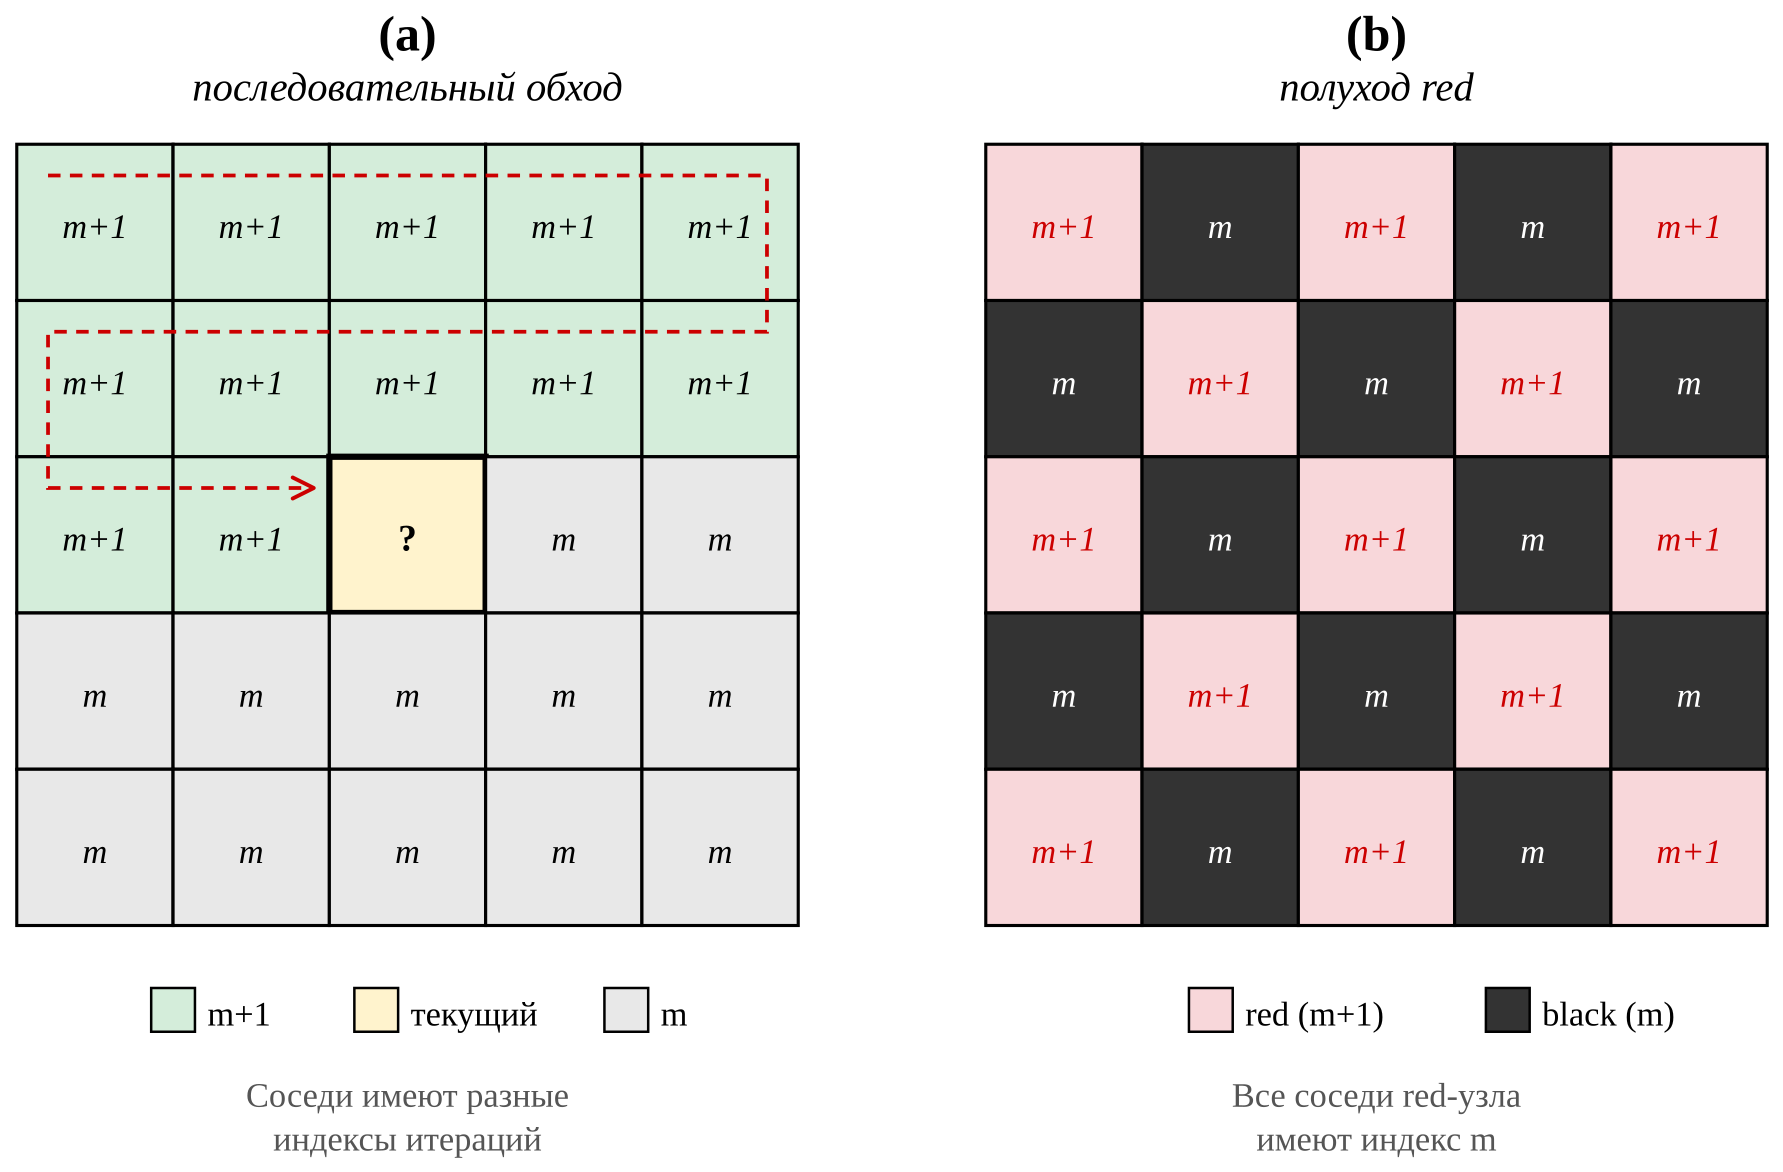
\includegraphics[width=\textwidth,height=0.9\textheight,keepaspectratio]{figures/ch03/fig_3_2.png}
\caption{Сравнение обхода сетки при обычном SOR и шахматной (Red--Black)
раскраске: (а)~последовательный обход по строкам смешивает индексы
итераций; (б)~полуход red обновляет только красные узлы, чёрные соседи
сохраняют индекс~$m$, что обеспечивает независимость обновлений}
\label{fig:rb_coloring}
\end{figure}

\FloatBarrier

Узлы с~$c = 0$ (условно «красные») и~$c = 1$ («чёрные») образуют два непересекающихся подмножества, покрывающих всю сетку. Название связано с аналогией шахматной доски: красные узлы занимают клетки одного цвета, чёрные~-- другого. Ключевое свойство раскраски состоит в том, что в пятиточечном шаблоне~\eqref{eq:5point_stencil} каждый красный узел имеет только чёрных соседей и наоборот. Поэтому при одновременном обновлении всех красных узлов каждый из них использует только значения чёрных соседей, которые не менялись на текущем полуходе,~-- все соседи имеют единый итерационный индекс (на полуходе red~-- индекс~$(m)$, на полуходе black~-- индекс~$(m+\tfrac{1}{2})$, см.\ формулы~\eqref{eq:rb_sor_red}-\eqref{eq:rb_sor_black}). Это свойство делает обновления внутри одного цвета полностью независимыми друг от друга и пригодными для массово-параллельного выполнения: каждый узел может обновляться отдельным потоком GPU без синхронизации с другими потоками. Синхронизация требуется только между полуходами и обеспечивается последовательным запуском ядер GPU: завершение ядра red гарантирует видимость обновлённых значений для ядра black (внутри одного ядра межпоточная синхронизация не требуется). Два полухода составляют одну полную итерацию.

\textit{Обновление давления на полуходе.}
В отличие от классического SOR~\eqref{eq:sor_update}, где часть соседних значений уже обновлена на текущей итерации (индексы~$(m)$ и~$(m+1)$ перемешаны), в Red-Black варианте обновление выполняется в два полухода с чёткой индексацией. На полуходе red обновляются узлы цвета~$c = 0$; их соседи (цвет~$c = 1$) сохраняют значения с итерации~$m$:
\begin{equation}\label{eq:rb_sor_red}
\begin{split}
  &\tilde{p}_{i,j} = \frac{1}{a_P}\bigl(
    a_E\,p_{i+1,j}^{(m)} + a_W\,p_{i-1,j}^{(m)}
    + a_N\,p_{i,j+1}^{(m)} + a_S\,p_{i,j-1}^{(m)}
    + b_{i,j}\bigr), \\
  &p_{i,j}^{(m+1/2)} = p_{i,j}^{(m)}
    + \omega\bigl(\tilde{p}_{i,j} - p_{i,j}^{(m)}\bigr),
    \qquad c(i,j) = 0.
\end{split}
\end{equation}

На полуходе black обновляются узлы цвета~$c = 1$; их соседи (цвет~$c = 0$) уже обновлены на текущей итерации и имеют индекс~$(m+1/2)$:
\begin{equation}\label{eq:rb_sor_black}
\begin{split}
  &\tilde{p}_{i,j} = \frac{1}{a_P}\bigl(
    a_E\,p_{i+1,j}^{(m+1/2)} + a_W\,p_{i-1,j}^{(m+1/2)} + \\
  &+ a_N\,p_{i,j+1}^{(m+1/2)} + a_S\,p_{i,j-1}^{(m+1/2)}
    + b_{i,j}\bigr), \\
  &p_{i,j}^{(m+1)} = p_{i,j}^{(m)}
    + \omega\bigl(\tilde{p}_{i,j} - p_{i,j}^{(m)}\bigr),
    \qquad c(i,j) = 1.
\end{split}
\end{equation}

Внутри каждого полухода все соседи имеют фиксированные значения (противоположный цвет не обновляется), что обеспечивает полную независимость обновлений и пригодность для массово-параллельного выполнения на GPU. Заметим, что на полуходе black релаксация в~\eqref{eq:rb_sor_black} выполняется от~$p_{i,j}^{(m)}$, поскольку чёрные узлы не затрагивались на полуходе red. В ядре обновления при необходимости выполняется проекция~$p \leftarrow \max(p,\, p_{\mathrm{cav}})$. В расчётах в избыточных давлениях обычно~$p_{\mathrm{cav}} = 0$. Проекция используется в режимах расчёта с кавитацией (условие Гюмбеля (half-Sommerfeld), раздел~3.5); в режиме полного заполнения может быть отключена.

\textit{Граничные условия на GPU.}
После каждой полной итерации (полуход red, затем полуход black) выполняется отдельное ядро, применяющее граничные условия из раздела~3.1. Внутренние узлы расположены в диапазоне~$i = 1, \ldots, N_z - 2$, $j = 1, \ldots, N_\varphi - 2$; слои~$j = 0$ и~$j = N_\varphi - 1$ используются как ghost-узлы для реализации периодичности, а строки~$i = 0$ и~$i = N_z - 1$ соответствуют торцевым границам с условиями Дирихле. Периодичность по окружному направлению обеспечивается копированием значений в ghost-узлы на границах: $P[i,\,0] = P[i,\,N_\varphi-2]$, $P[i,\,N_\varphi-1] = P[i,\,1]$. Это гарантирует корректное обращение к соседям при следующем полуходе. Условия Дирихле на торцах по оси~$z$ реализуются установкой давления кавитации: $P[0,\,j] = p_{\mathrm{cav}}$, $P[N_z-1,\,j] = p_{\mathrm{cav}}$. Граничные условия вынесены в отдельное ядро, чтобы не усложнять ветвление в основном ядре обновления. Это также упрощает адаптацию к другим типам граничных условий (например, при расчёте сектора вместо полного кольца). Ядро граничных условий запускается с одномерной сеткой потоков: каждый поток обрабатывает одну строку (для периодичности) или один столбец (для Дирихле).

\textit{Организация вычислений и конфигурация запуска.}
Ядро обновления давления использует двумерную сетку потоков GPU. Блок потоков имеет размер~$32 \times 8$: 32~потока по быстрому (окружному) индексу~$j$ соответствуют одной warp-линии~-- группе потоков, выполняющихся синхронно на одном мультипроцессоре. Такой выбор обеспечивает коалесцированный (последовательный) доступ к глобальной памяти: соседние потоки обращаются к соседним элементам массива, что минимизирует число транзакций памяти. Размер сетки блоков вычисляется из числа внутренних узлов: $(N_\varphi - 2)$ по окружному и $(N_z - 2)$ по осевому направлению. Потоки, попадающие за пределы расчётной области, завершаются без выполнения операций.

Каждый поток обрабатывает один внутренний узел. Поток вычисляет свои индексы~$(i,\,j)$ и проверяет условие раскраски~$c(i,j) = (i+j) \bmod 2$. Если цвет узла не совпадает с текущим полуходом, поток пропускает обновление. Все данные (давление, коэффициенты, правая часть) хранятся в глобальной памяти GPU в формате двойной точности. Коэффициенты дискретизации предварительно вычисляются на GPU из поля зазора~$h$ средствами поэлементных операций.

Ядро граничных условий запускается с одномерной сеткой потоков (блок из 256~потоков). Размер сетки определяется максимумом из~$N_z$ и~$N_\varphi$. Каждый поток обрабатывает либо одну строку (копирование для периодичности), либо один столбец (обнуление для Дирихле).

Коэффициенты дискретизации в реализации обозначаются~$A$, $B$, $C$, $D$, $E$, $F$ и связаны с обозначениями раздела~3.2 соотношениями: $A = a_E$, $B = a_W$, $C = a_N$, $D = a_S$, $E = a_P$, $F = b_{i,j}$.

\textit{Контроль сходимости.}
Сходимость контролируется по критерию относительной поправки~\eqref{eq:convergence_change} из раздела~3.3. Для снижения накладных расходов проверка выполняется не на каждой итерации, а с интервалом (типично~-- каждые несколько сотен итераций, таблица~\ref{tab:solver_params}). Перед началом блока итераций сохраняется копия текущего поля давления в отдельный GPU-буфер. После завершения блока вычисляется~$\delta^{(m)}$ средствами массовых операций GPU: поэлементное вычитание массивов, суммирование модулей разностей и суммирование модулей текущего решения. Эти операции выполняются на GPU без переноса данных на CPU; на CPU передаётся только скалярный результат~$\delta^{(m)}$. При $\delta^{(m)} < \varepsilon$ итерации прекращаются.

Проверка сходимости не на каждой итерации обусловлена тем, что вычисление~$\delta$ требует глобальной редукции (суммирования по всему массиву), которая является синхронной операцией и нарушает конвейер GPU. Выполнение редукции каждые несколько сотен итераций (а не каждую) практически не влияет на точность определения момента сходимости, но существенно снижает накладные расходы.

\textit{Кэширование GPU-буферов.}
При решении серии задач на одной сетке (например, параметрическое варьирование эксцентриситета, угла наклона, глубины микрорельефа) размер массивов не меняется. Выделение и освобождение GPU-памяти~-- дорогостоящие операции; повторное их выполнение на каждом вызове решателя создаёт значительные накладные расходы. Поэтому при первом вызове для данного размера сетки~$N_z \times N_\varphi$ выделяются рабочие буферы (массивы давления, копии для проверки сходимости, массивы коэффициентов дискретизации). При последующих вызовах с тем же размером сетки буферы переиспользуются~-- выполняется только обнуление массива давления и пересчёт коэффициентов. Это особенно эффективно при расчёте характеристик подшипника в диапазоне параметров, когда решатель вызывается десятки и сотни раз подряд.

\textit{Алгоритм итерации.}
На вход подаётся поле зазора~$h_{i,j}$, шаги сетки~$\Delta x_1$, $\Delta x_2$ и геометрические параметры ($R$,~$L$). На первом этапе из поля зазора вычисляются коэффициенты дискретизации~$a_E$, $a_W$, $a_N$, $a_S$, $a_P$ и правая часть~$b_{i,j}$~-- все операции выполняются на GPU. Поле давления инициализируется нулями.

Далее выполняется итерационный цикл. Одна полная итерация состоит из трёх этапов: обновление давления в узлах цвета~$c = 0$ (полуход red), обновление в узлах цвета~$c = 1$ (полуход black), применение граничных условий. С заданным интервалом (типично каждые 500~итераций) перед блоком итераций сохраняется копия поля давления, а после блока вычисляется относительная поправка~$\delta^{(m)}$~\eqref{eq:convergence_change}. Если $\delta^{(m)} < \varepsilon$, итерации прекращаются. Если достигнуто максимальное число итераций, процесс также останавливается с фиксацией достигнутого значения~$\delta$.

По завершении итераций результирующее поле давления переносится из памяти GPU на CPU для дальнейшего вычисления интегральных характеристик (несущая способность, момент трения, утечки; см.\ подраздел <<Целевые функционалы и выходные величины>>)~\cite{ansys2013}.

Описанный GPU-решатель применяется как внутренний решатель линейной системы в алгоритме JFO (раздел~3.5), где дополнительно выполняется обновление активного множества и вычисление степени заполнения~$\vartheta$ в кавитационной зоне.


\FloatBarrier
\section{Реализация модели кавитации JFO}
Теоретическая постановка задачи JFO (уравнение сохранения~\eqref{eq:jfo_conservation}, условия комплементарности~\eqref{eq:jfo_complementarity}) и общая схема итерационного алгоритма active-set приведены в подразделах~2.3.2-2.3.3~\cite{elrod1975}. В настоящем разделе описывается численная реализация каждого шага этого алгоритма: решение подсистемы для давления на GPU (раздел~3.4), обновление степени заполнения~$\vartheta$ в кавитационной зоне, переключение узлов между зонами полного заполнения и кавитации, критерии остановки. Алгоритм JFO имеет двухуровневую итерационную структуру: внутренний цикл~-- решение линейной системы для давления методом Red-Black SOR на GPU при фиксированном~$\vartheta$, внешний цикл~-- обновление активного множества и пересчёт~$\vartheta$.

\textit{Решение подсистемы для давления.}
На каждой внешней итерации~$m$ фиксируется текущее распределение~$\vartheta^{(m)}$. В узлах зоны полного заполнения ($\vartheta = 1$) решается система~\eqref{eq:5point_stencil} методом Red-Black SOR (раздел~3.4) до сходимости по критерию~\eqref{eq:convergence_change}. В узлах зоны кавитации давление фиксировано: $p_{i,j} = p_{\mathrm{cav}}$. Эти узлы не обновляются решателем давления; фиксация обеспечивается проекцией $p \leftarrow \max(p,\, p_{\mathrm{cav}})$, встроенной в ядро обновления (раздел~3.4). В кавитационных узлах давление фиксируется на уровне~$p_{\mathrm{cav}}$, поэтому внутри связной кавитационной области градиенты давления отсутствуют и напорный поток не формируется. На границе кавитации и полного заполнения градиент давления, как правило, отличен от нуля и определяется решением в зоне полного заполнения.

Коэффициенты напорной части дискретизации ($a_E$, $a_W$, $a_N$, $a_S$, $a_P$), определяемые полем зазора~$h$, не зависят от~$\vartheta$ и могут переиспользоваться во внутреннем цикле. Зависимость от~$\vartheta$ проявляется в переносном (куэттовском) потоке~\eqref{eq:flux_couette}, а также в классификации узлов как кавитационных ($p = p_{\mathrm{cav}}$) или полностью заполненных.

\textit{Обновление степени заполнения в кавитационной зоне.}
В кавитационной зоне $p = p_{\mathrm{cav}}$; внутри связной кавитационной области градиенты давления отсутствуют и напорный поток не формируется. Уравнение JFO~\eqref{eq:jfo_conservation} сводится к переносу массы куэттовским потоком. Для стационарной задачи это условие баланса переносных потоков:
\begin{equation}\label{eq:jfo_couette_balance}
  \frac{F_{C,\,i+\frac{1}{2},j} - F_{C,\,i-\frac{1}{2},j}}{\Delta x_1}
  + \frac{G_{C,\,i,j+\frac{1}{2}} - G_{C,\,i,j-\frac{1}{2}}}{\Delta x_2}
  = 0,
\end{equation}
\noindent где переносные потоки на гранях определены в~\eqref{eq:flux_couette} (раздел~3.2):
\begin{equation}\label{eq:jfo_theta_flux}
  F_{C,\,i+\frac{1}{2},j} = \frac{\vartheta_{\mathrm{up}}\,h_{i+\frac{1}{2},j}}{2}\,U_1,
  \quad
  G_{C,\,i,j+\frac{1}{2}} = \frac{\vartheta_{\mathrm{up}}\,h_{i,j+\frac{1}{2}}}{2}\,U_2.
\end{equation}

Значение~$\vartheta_{\mathrm{up}}$ берётся из наветренного узла по направлению скорости~$\mathbf{U}$ (upwind-схема, раздел~3.2). Толщина на грани~-- арифметическое среднее значений в соседних узлах.

В двумерной постановке соотношение~\eqref{eq:jfo_couette_balance} рассматривается как дискретное уравнение переноса для~$\vartheta$. Для наглядности приведём частный случай одномерного переноса по~$x_1$ при~$U_1 > 0$ и отсутствии потоков по~$x_2$, когда баланс упрощается и даёт явную рекуррентную связь:
\begin{equation}\label{eq:jfo_theta_update}
  \vartheta_{i,j} = \frac{\vartheta_{i-1,j}\,h_{i-\frac{1}{2},j}}
    {h_{i+\frac{1}{2},j}}.
\end{equation}

Это соотношение выражает сохранение массы при одномерном переносе: входящий куэттовский поток через грань~$i-1/2$ равен выходящему потоку через грань~$i+1/2$. В двумерном случае баланс~\eqref{eq:jfo_couette_balance} включает потоки по обоим направлениям и реализуется в виде дискретной схемы переноса для~$\vartheta$ (раздел~3.2).

Для нестационарного случая в узлах, отнесённых к кавитационной зоне, используется явная по времени схема (временной шаг~$\Delta t$ из~\eqref{eq:discrete_balance}):
\begin{equation}\label{eq:jfo_theta_transient}
\begin{split}
  &(\vartheta\,h)_{i,j}^{n+1} = (\vartheta\,h)_{i,j}^{n} - {} \\
  &- \Delta t \left[
    \frac{F_{C,\,i+\frac{1}{2},j} - F_{C,\,i-\frac{1}{2},j}}{\Delta x_1}
    + \frac{G_{C,\,i,j+\frac{1}{2}} - G_{C,\,i,j-\frac{1}{2}}}{\Delta x_2}
  \right].
\end{split}
\end{equation}

После обновления выполняется отсечка:
\[
  \vartheta_{i,j} := \min\bigl(1,\;\max(0,\;\vartheta_{i,j})\bigr).
\]

Отсечка обеспечивает физичность решения ($0 \leq \vartheta \leq 1$). Если~$\vartheta_{i,j}$ после обновления достигает единицы, узел переходит в зону полного заполнения на следующей внешней итерации.

\textit{Обновление активного множества.}
После решения подсистемы для давления и проекции $p \leftarrow \max(p,\, p_{\mathrm{cav}})$ каждый узел классифицируется: если $p_{i,j} > p_{\mathrm{cav}} + \varepsilon$, узел принадлежит зоне полного заполнения и~$\vartheta_{i,j} = 1$; если $p_{i,j} \leq p_{\mathrm{cav}} + \varepsilon$, узел принадлежит зоне кавитации и~$\vartheta_{i,j}$ обновляется из баланса переносных потоков~\eqref{eq:jfo_couette_balance}. Малый параметр~$\varepsilon$ (порядка $10^{-6}$-$10^{-8}$ в безразмерном давлении или относительно характерного масштаба давления) необходим для устойчивого определения зоны кавитации и предотвращения осцилляций активного множества на границе зон.

Переключение узлов между зонами~-- это и есть обновление активного множества. Узел может переходить из кавитации в полное заполнение (если~$\vartheta$ достигает~1 или давление вырастает выше~$p_{\mathrm{cav}}$) и обратно (если после проекции выполняется~$p_{i,j} \leq p_{\mathrm{cav}} + \varepsilon$). Процесс продолжается до стабилизации.

\textit{Двухуровневая итерационная структура.}
Внутренний уровень~-- решение линейной системы для давления методом Red-Black SOR на GPU (раздел~3.4) при фиксированном~$\vartheta$. Сходимость внутреннего цикла контролируется по критерию~\eqref{eq:convergence_change} с параметрами из таблицы~\ref{tab:solver_params}. Внешний уровень~-- итерации по активному множеству. На каждой внешней итерации последовательно выполняются: решение для давления (внутренний цикл), проекция~$p \geq p_{\mathrm{cav}}$, обновление активного множества, обновление~$\vartheta$ в кавитационной зоне, отсечка. Общая схема алгоритма приведена в подразделе~2.3.3 (см.\ также рисунок~\ref{fig:jfo_algorithm}).

\textit{Критерии остановки внешнего цикла.}
Внешние итерации прекращаются при одновременном выполнении двух условий: стабилизации активного множества (ни один узел не переключился между зонами на текущей итерации) и малости изменения решения ($\max_{i,j} |p_{i,j}^{(m+1)} - p_{i,j}^{(m)}| < \varepsilon_p$, $\max_{i,j} |\vartheta_{i,j}^{(m+1)} - \vartheta_{i,j}^{(m)}| < \varepsilon_\vartheta$; критерии сформулированы в подразделе~2.3.3). На практике стабилизация активного множества достигается за 5-20~внешних итераций (в зависимости от задачи), при этом каждая внешняя итерация содержит полный внутренний цикл GPU~SOR.

\textit{Инициализация.}
Начальное приближение: $p^{(0)}_{i,j} = p_{\mathrm{cav}}$, $\vartheta^{(0)}_{i,j} = 1$ (полное заполнение). При параметрических расчётах используется тёплый старт: решение предыдущей задачи как начальное приближение для~$p$ и~$\vartheta$, что существенно сокращает число как внешних, так и внутренних итераций.

Описанная реализация при консервативной аппроксимации потоков обеспечивает массосохраняющее решение задачи кавитации и применяется ко всем рассматриваемым постановкам (упорный и радиальный подшипники, возвратно-поступательная пара). Результаты расчётов приведены в главах~5--7.

\textit{Вычислительная стоимость JFO-реализации.}
Основная вычислительная стоимость JFO-алгоритма складывается из~двух частей. Первая~--- внутренний GPU~SOR-цикл для~решения задачи на~давление~--- по~трудоёмкости аналогична обычному решению уравнения Рейнольдса и~масштабируется как~$O(N_1 N_2)$ на~итерацию. Вторая~--- обновление активного множества и~степени заполнения~$\vartheta$~--- выполняется за~один проход по~сетке и~требует значительно меньших затрат. Суммарная стоимость одного внешнего цикла JFO примерно в~2--3~раза превышает стоимость одного SOR-цикла простой Reynolds-задачи; общее число внешних итераций обычно составляет 10--30. Таким образом, JFO-расчёт оказывается примерно в~20--60~раз дороже, чем~один прогон Reynolds-решателя с~обнулением давления. На~практике это приемлемо для~параметрических расчётов при~использовании тёплого старта.

\textit{Особенности сходимости при~фрагментированной кавитации на~микротекстуре.}
При~текстурированных поверхностях с~большим числом лунок (порядка~50--200 на~расчётную область) кавитационная картина существенно фрагментируется: каждая лунка содержит небольшую собственную кавитационную зону. Это замедляет сходимость внешнего цикла активного множества по~следующей причине: при~инициализации с~полным заполнением алгоритму необходимо последовательно <<выявить>> все~локальные кавитационные участки, причём в~начале итераций граница одной кавитационной зоны может влиять на~соседние через~поле давления. Число внешних итераций в~этом случае может вырастать до~50--100 по~сравнению с~10--15 для~гладкого подшипника. Использование тёплого старта существенно снижает этот эффект: при~близких параметрах кавитационный рисунок от~предыдущего решения уже достаточно близок к~текущему, и~алгоритм сходится за~5--15 внешних итераций.

\textit{Допущение о~фиксированной кавитационной области в~динамике.}
При~расчёте динамических коэффициентов (раздел~4.4, глава~8) для~каждого набора возмущений $(\xi, \eta, \dot\xi, \dot\eta)$ в~принципе необходимо решать полную задачу JFO, в~том числе заново определять границу кавитации. Однако это многократно увеличивает вычислительные затраты. На~практике применяется допущение о~фиксированной кавитационной области (\textit{frozen cavitation}): граница кавитации берётся по~полю равновесного давления~$P_0$ и~при~решении возмущённой задачи не~пересматривается. Это допущение оправдано при~малых амплитудах возмущений~$|\xi|, |\eta| \ll c$ и~обеспечивает разумную точность для~прямых коэффициентов. Для~перекрёстных коэффициентов погрешность может быть заметнее, особенно в~режимах с~обширной кавитационной зоной.

\textit{Вычислительная стоимость JFO-реализации.}
Основная вычислительная стоимость JFO-алгоритма складывается из~двух частей. Первая~--- внутренний GPU~SOR-цикл для~решения задачи на~давление~--- по~трудоёмкости аналогична обычному решению уравнения Рейнольдса и~масштабируется как~$O(N_1 N_2)$ на~итерацию. Вторая~--- обновление активного множества и~степени заполнения~$\vartheta$~--- выполняется за~один проход по~сетке и~требует значительно меньших затрат. Суммарная стоимость одного внешнего цикла JFO примерно в~2--3~раза превышает стоимость одного SOR-цикла простой Reynolds-задачи; общее число внешних итераций обычно составляет 10--30. Таким образом, JFO-расчёт оказывается примерно в~20--60~раз дороже, чем~один прогон Reynolds-решателя с~обнулением давления. На~практике это приемлемо для~параметрических расчётов при~использовании тёплого старта.

\textit{Особенности сходимости при~фрагментированной кавитации на~микротекстуре.}
При~текстурированных поверхностях с~большим числом лунок (порядка~50--200 на~расчётную область) кавитационная картина существенно фрагментируется: каждая лунка содержит небольшую собственную кавитационную зону. Это замедляет сходимость внешнего цикла активного множества по~следующей причине: при~инициализации с~полным заполнением алгоритму необходимо последовательно <<выявить>> все~локальные кавитационные участки, причём в~начале итераций граница одной кавитационной зоны может влиять на~соседние через~поле давления. Число внешних итераций в~этом случае может вырастать до~50--100 по~сравнению с~10--15 для~гладкого подшипника. Использование тёплого старта существенно снижает этот эффект: при~близких параметрах кавитационный рисунок от~предыдущего решения уже достаточно близок к~текущему, и~алгоритм сходится за~5--15 внешних итераций.

\textit{Допущение о~фиксированной кавитационной области в~динамике.}
При~расчёте динамических коэффициентов (раздел~4.4, глава~8) для~каждого набора возмущений $(\xi, \eta, \dot\xi, \dot\eta)$ в~принципе необходимо решать полную задачу JFO, в~том числе заново определять границу кавитации. Однако это многократно увеличивает вычислительные затраты. На~практике применяется допущение о~фиксированной кавитационной области (\textit{frozen cavitation}): граница кавитации берётся по~полю равновесного давления~$P_0$ и~при~решении возмущённой задачи не~пересматривается. Это допущение оправдано при~малых амплитудах возмущений~$|\xi|, |\eta| \ll c$ и~обеспечивает разумную точность для~прямых коэффициентов. Для~перекрёстных коэффициентов погрешность может быть заметнее, особенно в~режимах с~обширной кавитационной зоной.


% \FloatBarrier
% \FloatBarrier
\section*{Выводы по главе 3}
\phantomsection\addcontentsline{toc}{section}{Выводы по главе 3}

В главе~3 описана численная реализация решения задач гидродинамики
смазочного слоя, включая дискретизацию уравнения Рейнольдса,
итерационные методы, GPU-ускорение и реализацию модели кавитации JFO.

\begin{enumerate}[wide, labelindent=\parindent, nosep]
  \item Сформулированы граничные условия для дискретной задачи:
    условия Дирихле ($p = p_{\mathrm{cav}}$) на открытых границах,
    периодичность по окружному направлению (в частности, через ghost-узлы
    в GPU-реализации), условия Неймана при расчёте сектора.
    В реализации граничные условия выделены в отдельный этап.
  \item Выполнена консервативная дискретизация уравнения Рейнольдса
    на основе баланса потоков через грани контрольного объёма.
    Напорные потоки аппроксимированы центральными разностями
    (второй порядок), а переносная часть в постановке JFO
    (перенос $\vartheta$) реализована upwind-схемой первого порядка,
    обеспечивающей устойчивость при доминировании конвективного переноса.
    Дискретизация для давления (при $\vartheta=1$) приводит к линейной
    системе с пятиточечным шаблоном.
  \item Для решения дискретной системы выбран метод последовательной
    верхней релаксации (SOR) как естественное ускорение метода
    Гаусса--Зейделя.  Сформулированы критерии сходимости
    (относительная поправка и невязка разностного уравнения)
    и определены параметры итерационного процесса.
  \item Для преодоления ограничения последовательного SOR
    на параллелизм реализован метод Red-Black SOR на GPU.
    Шахматная раскраска сетки и двухполуходная схема (red/black)
    обеспечивают независимость обновлений внутри полухода, что позволяет
    эффективно использовать массово-параллельную архитектуру GPU.
    Описаны конфигурация запуска ядер, кэширование GPU-буферов для серийных
    расчётов и механизм контроля сходимости с минимальными накладными
    расходами на глобальную редукцию.
  \item Реализован алгоритм решения задачи кавитации JFO
    с двухуровневой итерационной структурой: внутренний цикл
    (GPU Red-Black SOR для давления при фиксированном~$\vartheta$)
    и внешний цикл (обновление активного множества и пересчёт степени
    заполнения~$\vartheta$ из баланса переносных потоков).
    Обновление~$\vartheta$ в кавитационной зоне основано на дискретном
    уравнении переноса куэттовским потоком с upwind-аппроксимацией.
    Реализация при консервативной аппроксимации потоков обеспечивает
    массосохраняющее решение задачи кавитации.
\end{enumerate}

Разработанный вычислительный алгоритм (дискретизация, GPU-решатель, JFO)
применяется ко всем рассматриваемым постановкам (упорный, радиальный
и возвратно-поступательный подшипники) и используется в расчётах,
представленных в последующих главах.


\FloatBarrier
\section*{Контрольные вопросы}
\phantomsection\addcontentsline{toc}{section}{Контрольные вопросы}

\begin{enumerate}
\item Какие граничные условия используются для~уравнения Рейнольдса?
\item В~чём суть метода конечных разностей применительно к~уравнению Рейнольдса?
\item Чем~отличаются итерационные методы Якоби и~Гаусса--Зейделя?
\item Что~такое метод верхней релаксации (SOR) и~как выбирается параметр релаксации?
\item В~чём преимущества GPU-реализации вычислений?
\item Что~такое алгоритм Red--Black SOR и~почему он~подходит для~параллельных вычислений?
\item Как~реализуется модель кавитации JFO в~численной схеме?
\item Какие критерии сходимости используются при~итерационном решении?
\item Что~такое метод тёплого старта и~в~каких случаях он~эффективен?
\item В~чём преимущества консервативной дискретизации для~задач с~кавитацией?
\end{enumerate}
